\documentclass[tikz,border=10pt]{standalone}
\usepackage{tikz}
\usetikzlibrary{arrows.meta,calc}

\definecolor{figazul}{RGB}{2,132,199}
\definecolor{figrojo}{RGB}{220,38,38}
\definecolor{figverde}{RGB}{22,163,74}

\begin{document}
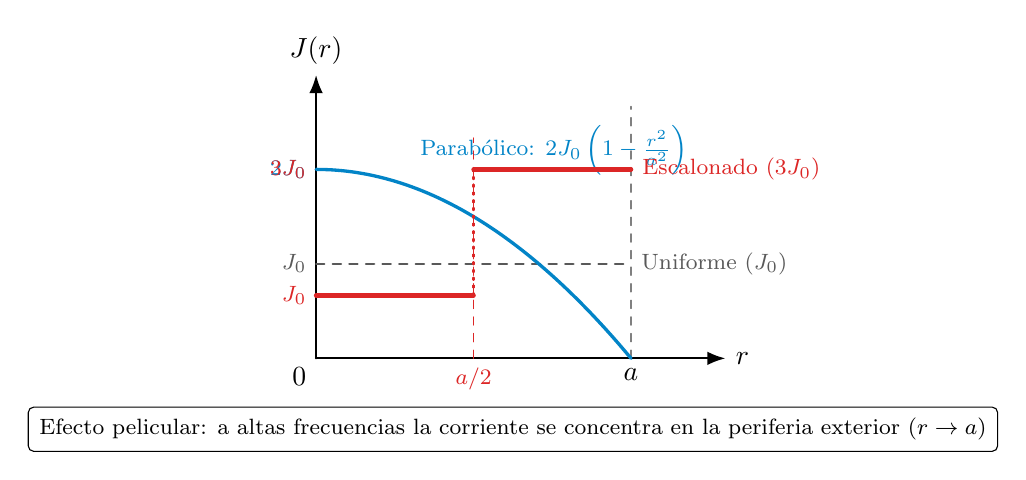
\begin{tikzpicture}[>=Latex, line cap=round, line join=round]
  % Ejes de coordenadas
  \draw[->, thick] (0,0) -- (5.2,0) node[right] {$r$};
  \draw[->, thick] (0,0) -- (0,3.6) node[above] {$J(r)$};
  \node[below left] at (0,0) {$0$};

  % Cota del radio a en el eje horizontal
  \draw[dashed, thin, color=gray] (4.0, 0) -- (4.0, 3.2);
  \node[below, color=black] at (4.0, 0) {$a$};

  % 1. Perfil Uniforme: J(r) = J_0
  \draw[thick, color=gray!70!black, dashed] (0, 1.2) -- (4.0, 1.2) node[right, font=\footnotesize, color=gray!70!black] {Uniforme ($J_0$)};
  \node[left, font=\footnotesize, color=gray!70!black] at (0, 1.2) {$J_0$};

  % 2. Perfil Parabólico: J(r) = 2J_0 (1 - r^2 / a^2)
  \draw[domain=0:4.0, smooth, variable=\x, very thick, color=figazul] 
    plot ({\x}, {2.4 * (1 - (\x/4.0)*(\x/4.0))});
  \node[above right, font=\footnotesize, color=figazul] at (1.2, 2.2) 
    {Parabólico: $2J_0\left(1 - \frac{r^2}{a^2}\right)$};
  \node[left, font=\footnotesize, color=figazul] at (0, 2.4) {$2J_0$};

  % 3. Perfil Escalonado: J0 para r < R/2, 3J0 para r > R/2
  \draw[dashed, thin, color=figrojo] (2.0, 0) -- (2.0, 2.8);
  \node[below, font=\footnotesize, color=figrojo] at (2.0, 0) {$a/2$};
  \draw[ultra thick, color=figrojo] (0, 0.8) -- (2.0, 0.8);
  \draw[dotted, thick, color=figrojo] (2.0, 0.8) -- (2.0, 2.4);
  \draw[ultra thick, color=figrojo] (2.0, 2.4) -- (4.0, 2.4) node[right, font=\footnotesize, color=figrojo] {Escalonado ($3J_0$)};
  \node[left, font=\footnotesize, color=figrojo] at (0, 0.8) {$J_0$};
  \node[left, font=\footnotesize, color=figrojo] at (0, 2.4) {$3J_0$};

  % Cartel explicativo
  \node[draw, rounded corners=2pt, inner sep=4pt, fill=white, fill opacity=0.9, text opacity=1, font=\footnotesize] at (2.5, -0.9)
    {Efecto pelicular: a altas frecuencias la corriente se concentra en la periferia exterior ($r \to a$)};
\end{tikzpicture}
\end{document}
